\section{高维球谐与对称无迹张量}
\label{sec:ghs-harmonics-stf}

三维角动量耦合把张量分解为不可约分量，但直接列举磁量子数并不适合任意维数。
将完全对称张量编码为齐次多项式后，取迹变成一次 Laplace 运算，去迹因而可以用统一的递推完成。
这一构造同时给出 $SO(d)$ 的球面角模态和后文共形初级态所需的旋转表示。
以下 $d>2$，坐标与辅助极化向量均无量纲；物理角动量算符仍须乘以 $\hbar$。

\begin{definition}[齐次多项式与调和张量]
在 $\RR^d$ 中令 $\mathcal P_S$ 为 $S$ 次齐次多项式的空间，$\mathcal H_S=\ker\Delta_{\RR^d}\cap\mathcal P_S$。由恒等式 $\Delta(r^2Q)=2(d+2k)Q+r^2\Delta Q$ 对次数为 $k$ 的 $Q$ 成立，这是下面分解的关键。
\end{definition}

\begin{theorem}[调和分解与球谐维数]
\label{thm:ghs-harmonic-polynomial-decomposition}
对 $d>2$ 与整数 $S\geq 0$，存在 $SO(d)$ 不变的直和分解
\begin{equation}\label{eq:ghs-harmonic-direct-sum}
 \mathcal P_S=\mathcal H_S\oplus r^2\mathcal P_{S-2},
\end{equation}
其中 $\mathcal P_{k}=\{0\}$ 当 $k<0$，负下标二项式系数取零。于是
\begin{equation}\label{eq:ghs-dim-harmonic-polynomial}
 \dim\mathcal H_S=\binom{S+d-1}{S}-\binom{S+d-3}{S-2}.
\end{equation}
\end{theorem}
\begin{proof}
令 $\mathcal P_S$ 上的 Fischer 内积为
$\langle P,Q\rangle_F=[\overline{P}(\partial)Q(x)]_{x=0}$，其中
$\overline{P}(\partial)$ 表示把 $\overline P$ 的每个变量 $x^i$ 换为 $\partial_i$。对单项式 $x^\alpha$，该内积等于 $\alpha!$，故正定。乘以 $r^2=\sum_i(x^i)^2$ 的伴随正好是 $\Delta=\sum_i\partial_i^2$，即对 $P\in\mathcal P_S,Q\in\mathcal P_{S-2}$ 有
\[
 \langle P,r^2Q\rangle_F=\langle\Delta P,Q\rangle_F.
\]
因此 $(r^2\mathcal P_{S-2})^\perp=\ker\Delta\cap\mathcal P_S=\mathcal H_S$。有限维 Hilbert 空间的正交分解给出
$\mathcal P_S=\mathcal H_S\oplus r^2\mathcal P_{S-2}$，无需猜测去迹系数。乘以 $r^2$ 是单射，所以
$\dim(r^2\mathcal P_{S-2})=\dim\mathcal P_{S-2}$。又 $\dim\mathcal P_k=\binom{k+d-1}{k}$，两维数相减即得公式。
\end{proof}

\begin{proposition}[张量的迹与球谐谱]
完全对称张量 $T_{i_1\cdots i_S}$ 与齐次多项式
$P_T(x)=T_{i_1\cdots i_S}x^{i_1}\cdots x^{i_S}$ 一一对应。
其迹满足
\[
 \Delta P_T=S(S-1)T^j{}_{j i_3\cdots i_S}x^{i_3}\cdots x^{i_S}.
\]
因此调和多项式恰对应对称无迹张量。
若 $P_T(rn)=r^SY_T(n)$ 调和，则单位球面的正 Laplace 算子满足
\begin{equation}\label{eq:ghs-spherical-harmonic-casimir}
 -\Delta_{S^{d-1}}Y_T=S(S+d-2)Y_T.
\end{equation}
\end{proposition}
\begin{proof}
第一次求导可以落在 $S$ 个相同的对称指标上，第二次可以落在剩余的 $S-1$ 个上，
缩并两次求导的指标便给出系数 $S(S-1)$。当 $S<2$ 时取迹自动为零。
在极坐标中，欧氏 Laplace 算子是
\[
 \Delta_{\RR^d}=\partial_r^2+\frac{d-1}{r}\partial_r+\frac1{r^2}\Delta_{S^{d-1}}.
\]
代入 $r^SY_T$，径向两项合为 $S(S+d-2)r^{S-2}Y_T$。
调和条件将其与角向项相抵消，得到\eqnrefs{eq:ghs-spherical-harmonic-casimir}。
\end{proof}

局部张量秩 $S$ 与球谐次数 $S$ 在这个构造中相联系。
这个联系用到了欧氏空间的全局正交群，不对任意背景自动成立。

\begin{figure}[htbp]
\centering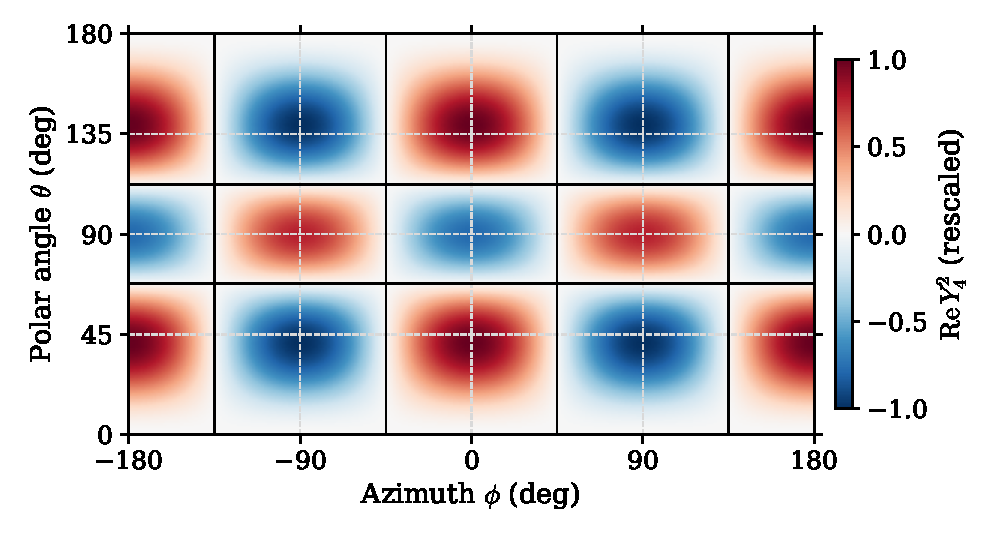
\includegraphics[width=.79\linewidth]{content/GroupTheory/figures/geometry-highspin/generated/spherical_harmonic_nodal.pdf}
\caption{球面调和函数 $\operatorname{Re}Y_4^2$ 的经纬坐标图（整体幅度重新归一）：红、蓝表示不同符号，黑线表示节点。球面坐标的接缝和两极只是参数化现象，不是波函数奇点。}\label{fig:ghs-spherical-harmonic-nodal}
\end{figure}

\cref{fig:ghs-spherical-harmonic-nodal} 把抽象的 $SO(3)$ 不可约表示变成可检查的几何对象；相同的 $\ell$ 可对应不同 $m$ 的角模式，而非单一的“自旋方向”。

\begin{proposition}[一般齐次多项式的调和投影]
若 $P$ 为 $S$ 次齐次多项式，定义
\[
 H(P)=\sum_{k=0}^{\lfloor S/2\rfloor}
 \frac{(-1)^k r^{2k}\Delta^kP}
 {4^k k!\prod_{j=1}^k(S+d/2-1-j)}.
\]
它满足 $\Delta H(P)=0$ 且 $P-H(P)\in r^2\mathcal P_{S-2}$，所以是上述直和分解的调和投影。
\end{proposition}
\begin{proof}
逐项使用乘积法则与 Euler 齐次恒等式 $x\cdot\partial Q_q=qQ_q$，得到
\[
 \Delta(r^{2k}Q_q)=2k(2q+d+2k-2)r^{2k-2}Q_q+r^{2k}\Delta Q_q,
\]
这里 $Q_q$ 是 $q$ 次齐次多项式。取 $q=S-2k$，相邻两项的系数恰好抵消，因此 $\Delta H(P)=0$。

最低阶 $S=2$ 给出 $H(P)=P-r^2\Delta P/(2d)$，即矩阵的标准去迹公式。无需先假定 Gegenbauer 多项式，此法已经为任意阶张量提供算法。
\end{proof}

\subsection{双边无迹投影与系数递推}

\begin{definition}[对称张量的极化编码]
在 $d>2$ 维欧氏空间，令 $T_{\mu_1\cdots\mu_S}$ 是秩 $S$ 的完全对称张量。把它编码为齐次多项式 $T(z)=T_{\mu_1\cdots\mu_S}z^{\mu_1}\cdots z^{\mu_S}$。无迹条件等价于 $\partial_z^2T(z)=0$。

对于任意两个向量 $z,w$，要从 $(z\cdot w)^S$ 中抽取双边对称无迹部分，就必须减去所有含 $z^2$ 或 $w^2$ 的迹项。
\end{definition}

\begin{theorem}[对称无迹张量的投影多项式]
设 $\nu=(d-2)/2$，升阶乘为 $(a)_S=\Gamma(a+S)/\Gamma(a)$。
Gegenbauer 多项式 $C_S^{(\nu)}(t)$ 由生成函数
$(1-2ut+u^2)^{-\nu}=\sum_{S\geq0}C_S^{(\nu)}(t)u^S$ 定义。
无迹投影的闭式表达为
\begin{equation}\label{eq:ghs-r4-stf-projector}
 \mathcal P_S(z,w)=\frac{S!}{2^S(\nu)_S}
 (z^2w^2)^{S/2}
 C_S^{(\nu)}\!\left(\frac{z\cdot w}{\sqrt{z^2w^2}}\right),
 \qquad S\ge0.
\end{equation}
右侧理解为多项式恒等式，故 $z^2=0$ 或 $w^2=0$ 时可直接以展开后得到的多项式求值，而不需要真的计算分母。该多项式分别对 $z,w$ 调和，而且最高次不含迹项的系数为一。
\end{theorem}
\begin{proof}
不必先知道 Gegenbauer 多项式，也可以从零开始求出全部系数。把关于 $z$ 和 $w$ 都齐次 $S$ 次的候选多项式写作
\[
 P_S(z,w)=\sum_{k=0}^{\lfloor S/2\rfloor}
 a_k(z^2w^2)^k(z\cdot w)^{S-2k},\qquad a_0=1.
\]
设 $m=S-2k$。先对每一项按乘积法则求一次 Laplace 算符：
\begin{align*}
 \partial_z^2\bigl[(z^2)^k(z\cdot w)^m\bigr]
 &=2k(d+2m+2k-2)(z^2)^{k-1}(z\cdot w)^m\\
 &\quad +m(m-1)w^2(z^2)^k(z\cdot w)^{m-2}.
\end{align*}
第一项在 $k\mapsto k+1$ 后和第二项具有相同的单项式。要求它们的系数逐项相消，得到
\begin{equation}\label{eq:ghs-r12-stf-recursion}
 a_{k+1}=-\frac{(S-2k)(S-2k-1)}{2(k+1)(d+2S-2k-4)}\,a_k.
\end{equation}
特别地，$a_1=-S(S-1)/[2(d+2S-4)]$。当 $S=2$ 时等于 $-1/d$，当 $S=3$ 时等于 $-3/(d+2)$，从而逐项恢复低自旋的无迹投影。递推也可写成
\[
 a_k=\frac{(-1)^k S!\,\Gamma(S+d/2-1-k)}
 {4^k k!(S-2k)!\,\Gamma(S+d/2-1)},
\]
因为相邻 Gamma 函数之比恰好给出 \cref{eq:ghs-r12-stf-recursion}。此式与 Gegenbauer 表示相等，但现在每个迹补偿系数都有了可以核对的来源。


令 $t=(z\cdot w)/\sqrt{z^2w^2}$，写 $\mathcal P_S(z,w)=(z^2w^2)^{S/2}f_S(t)$。把 $z$ 当成自变量并使用 $d$ 维 Laplace 算符的径向分解，调和条件化为
\begin{equation*}
 (1-t^2)f_S''(t)-(d-1)t f_S'(t)+S(S+d-2)f_S(t)=0.
\end{equation*}
取 $2\nu+1=d-1$，这就是 Gegenbauer 微分方程，因此多项式解为 $f_S(t)=A_SC_S^{(\nu)}(t)$。由生成函数
\begin{equation*}
 (1-2ut+u^2)^{-\nu}=\sum_{S=0}^\infty C_S^{(\nu)}(t)u^S
\end{equation*}
可知 $C_S^{(\nu)}(t)$ 的最高次系数为 $2^S(\nu)_S/S!$。选择 $A_S=S!/[2^S(\nu)_S]$，就使 $\mathcal P_S$ 中 $(z\cdot w)^S$ 的系数恰好等于一。$z$ 与 $w$ 的对称性进一步保证对 $w$ 的调和条件也自动满足。
\end{proof}

\begin{example}[秩零至秩三的迹补偿]
将对称无迹极化核的一般公式用于秩 $S=0,1,2,3$，明确写出各阶迹补偿项。

\textbf{解。} \begin{align}\label{eq:ghs-r4-stf-lowspin}
 \mathcal P_0(z,w)&=1,\qquad \mathcal P_1(z,w)=z\cdot w,\\
 \mathcal P_2(z,w)&=(z\cdot w)^2-\frac{z^2w^2}{d},\notag\\
 \mathcal P_3(z,w)&=(z\cdot w)^3-\frac{3z^2w^2(z\cdot w)}{d+2}.\notag
\end{align}
特别地，自旋二的迹减除系数是 $1/d$，不是随意选取的 $1/(d-1)$。这也解释了为何零极化方式在求相关函数时简洁，而在计算散度前必须恢复与任意 $z$ 相容的迹结构。
\end{example}

\subsection{零极化等价类上的微分}

由调和直和分解，每个模掉 $z^2$ 倍数的多项式等价类都有唯一调和代表。因此一个作用在其等价类上的微分算符就不能对不同的代表给出不同结果。普通 $\partial/\partial z^\mu$ 不满足这一要求，因为 $\partial_{z^\mu}(z^2f)$ 含有 $2z_\mu f$。因此需要一个保持 $z^2$ 倍数所构成理想的微分算符。

\begin{definition}[Thomas 导数]
设 $\nu=(d-2)/2$，定义
\begin{equation}\label{eq:ghs-r4-thomas-restated}
 \mathscr D_{z,\mu}=\left(\nu+z\cdot\partial_z\right)\partial_{z^\mu}
 -\frac12z_\mu\partial_z^2.
\end{equation}
\end{definition}

\begin{proposition}[Thomas 导数保持迹理想]
对次数为 $m$ 的任意齐次多项式 $f_m$，直接展开可得
\begin{equation}\label{eq:ghs-r4-thomas-ideal}
 \mathscr D_{z,\mu}(z^2f_m)=z^2(\cdots)_\mu.
\end{equation}
因此在 $z^2=0$ 上，$\mathscr D_z$ 只依赖张量的对称无迹等价类。
\end{proposition}
\begin{proof}
当 $f_m$ 的齐次次数为 $m$ 时，直接对乘积求导得
\begin{align*}
 \partial_{z^\mu}(z^2f_m)&=2z_\mu f_m+z^2\partial_{z^\mu}f_m,\\
 \partial_z^2(z^2f_m)&=(2d+4m)f_m+z^2\partial_z^2f_m.
\end{align*}
把两行代回 \cref{eq:ghs-r4-thomas-restated}，不含 $z^2$ 的项合为
\begin{equation*}
 \bigl[2(\nu+m+1)-(d+2m)\bigr]z_\mu f_m=0,
\end{equation*}
因为 $2\nu=d-2$。余下各项全部含显式的 $z^2$ 因子，从而证明 \cref{eq:ghs-r4-thomas-ideal}。此证明不要求事先指定 $f_m$ 的迹，所以适用于任意秩无迹张量的所有代表。
\end{proof}

\begin{example}[Thomas 导数作用于单项极化张量]
计算 Thomas 导数作用于单项极化多项式 $(z\cdot w)^S$ 的结果，并核对它与取迹之间的关系。

\textbf{解。} 由乘积法则与 $z\cdot\partial_z(z\cdot w)^{S-1}=(S-1)(z\cdot w)^{S-1}$ 得
\begin{align}\label{eq:ghs-r4-thomas-action}
 &\mathscr D_{z,\mu}(z\cdot w)^S\\
 &\quad=S(\nu+S-1)w_\mu(z\cdot w)^{S-1}
 -\frac{S(S-1)}2z_\mu w^2(z\cdot w)^{S-2}.\notag
\end{align}
当 $w^2=0$ 时只留下第一项；当 $w^2\ne0$ 时，第二项是不可遗漏的迹补偿。对于秩 $S$ 对称无迹算符 $J_S(x,z)$，$\partial_x\cdot\mathscr D_z$ 因而能定义一个与极化代表无关的散度多项式。真正物理散度的规范因子需按 $S(\nu+S-1)$ 等最高权系数确定，不宜在改变张量编码约定时直接照搬。这一结构也为相互作用流的散度计算提供无歧义的定义。
\end{example}

\subsection{最高权球谐的积分归一化}

复零极化 $a=(1,\ii,0,\ldots,0)$ 满足 $a\cdot a=0$，
所以 $(a\cdot x)^k$ 调和。限制到单位球面后，令 $z=a\cdot n=n^1+\ii n^2$，
它在第一、第二坐标平面的转动下获得相位 $\ee^{\ii k\alpha}$。
要把这些角模式用于态空间，必须确定它们的范数，而不能只知道其转动权。

\begin{proposition}[复零极化球谐的范数]
\label{prop:ghs-highest-harmonic-integral}
对于 $d>2$、整数 $k,j\geq0$，令 $\Omega_{d-1}=2\pi^{d/2}/\Gamma(d/2)$，则
\begin{equation}\label{eq:ghs-highest-harmonic-integral}
 \int_{S^{d-1}}z^k\bar z^j\,\dd\Omega
 =\delta_{kj}\Omega_{d-1}\frac{k!}{(d/2)_k},
 \qquad (a)_k=\frac{\Gamma(a+k)}{\Gamma(a)}.
\end{equation}
\end{proposition}
\begin{proof}
取 $d$ 个独立、同方差的实 高斯随机变量 $X_i$。
向量 $n=X/|X|$ 的分布旋转不变，故是球面均匀测度。
令 $U=(X_1^2+X_2^2)/2$、$V=\sum_{i=3}^dX_i^2/2$，
在单位方差的选择下它们分别具有形状参数 $1$、$(d-2)/2$ 的独立 Gamma 密度。
变量替换 $U=rs,V=r(1-s)$ 的 Jacobian 是 $r$，因此
\[
 f_{r,s}(r,s)=\frac{\ee^{-r}r^{d/2-1}}{\Gamma((d-2)/2)}
 (1-s)^{(d-2)/2-1},\quad r>0,\quad0<s<1.
\]
对 $r$ 积分得到 $s=|z|^2$ 的贝塔密度；其 $k$ 阶矩为
\begin{align*}
 \int_{S^{d-1}}\dd\Omega\,|z|^{2k}
 &=\Omega_{d-1}\frac{B(k+1,(d-2)/2)}{B(1,(d-2)/2)}\\
 &=\Omega_{d-1}\frac{\Gamma(k+1)\Gamma(d/2)}{\Gamma(k+d/2)}
 =\Omega_{d-1}\frac{k!}{(d/2)_k}.
\end{align*}
转动 $z\mapsto\ee^{\ii\alpha}z$ 保持球面测度，故非对角积分等于自身乘以
$\ee^{\ii(k-j)\alpha}$。当 $k\ne j$ 时选择这个相位不为一的 $\alpha$，便得到积分为零。
\end{proof}

\begin{example}[四维最高权模式]
在 $d=4$ 的单位球面上，归一化最高权标量模式 $z^k$，并核对不同最高权阶数之间的角向正交性。

\textbf{解。} 当 $d=4$ 时，$\Omega_3=2\pi^2$、$(2)_k=(k+1)!$，故
\[
 N_{4,k}=\int_{S^3}|z|^{2k}\,\dd\Omega=\frac{2\pi^2}{k+1},
 \qquad Y_k(n)=\sqrt{\frac{k+1}{2\pi^2}}\,z^k.
\]
归一化后 $\langle Y_j,Y_k\rangle=\delta_{jk}$。径向量子化中的双粒子模式还需各自的频率与玻色归一化，
角积分本身只确定这里的一粒子角向正交性。
\end{example}

完全对称张量的去迹与球谐的调和条件由同一算子控制。
因此三维的不可约张量方法可以在任意 $d>2$ 维继续使用；改变的是旋转群和维数，
而不是张量矩阵元必须先分解不可约分量这一原则。
